\section{Results}
\label{sec:results}
We consider 3 aspects of bug hunting:

\begin{enumerate}
  \item The Evolution of Incentives for each bug bounty program, starting from its launch time (and given already existing programs)
  \item The individual contributions by security researchers to bounty programs, and how these contributions are affected by newly launched programs
  \item How individual security researchers compound their cumulative payoff across a variety of bounty programs.
\end{enumerate}

\subsection{Considering a specific participant in a specific program}
In the former section, we considered bounty programs at the aggregate level.


%\begin{figure}
%\begin{center}
%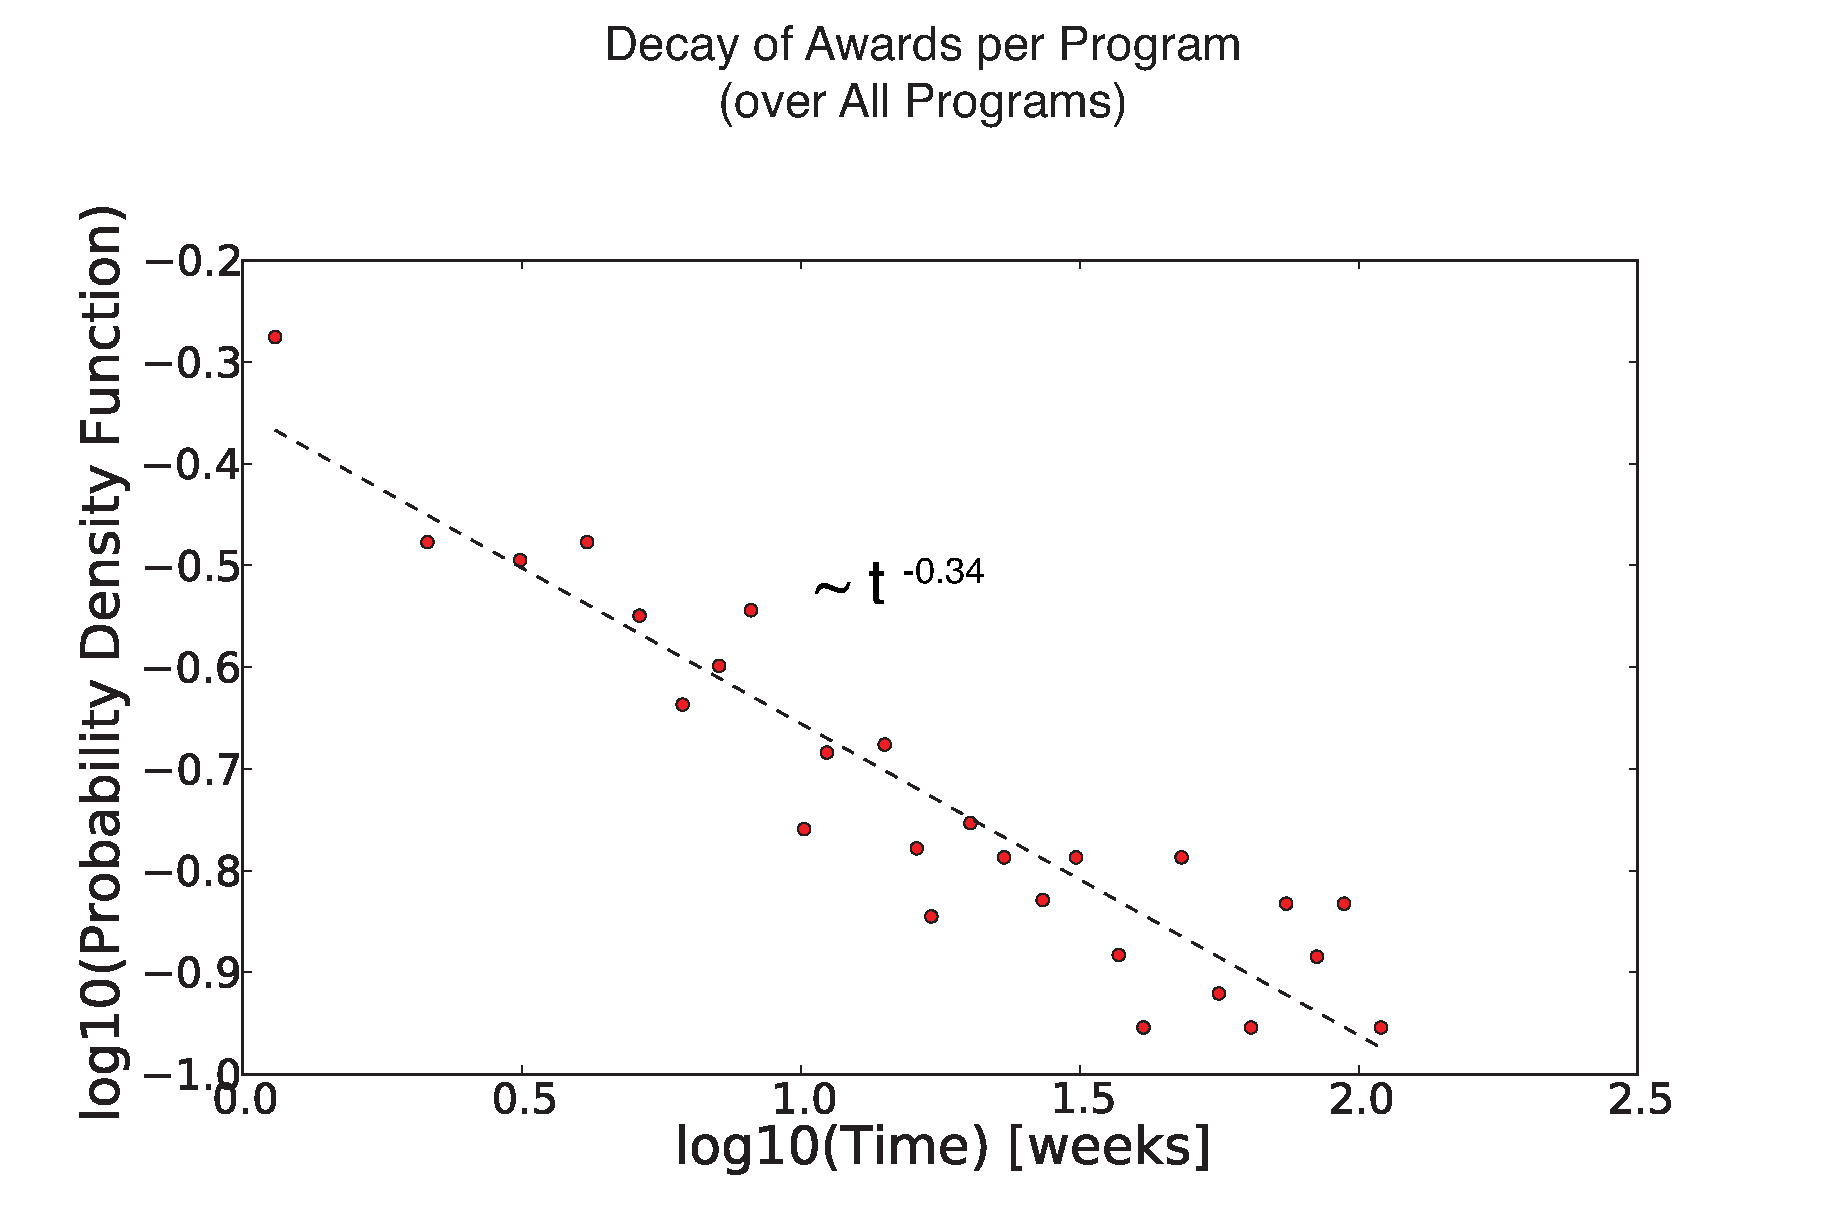
\includegraphics[width=10cm]{figures/decay.eps}
%\caption{Probability density function of vulnerability discovery as a function of time}
%\label{fig:decay}
%\end{center}
%\end{figure}


\begin{figure}
\begin{center}
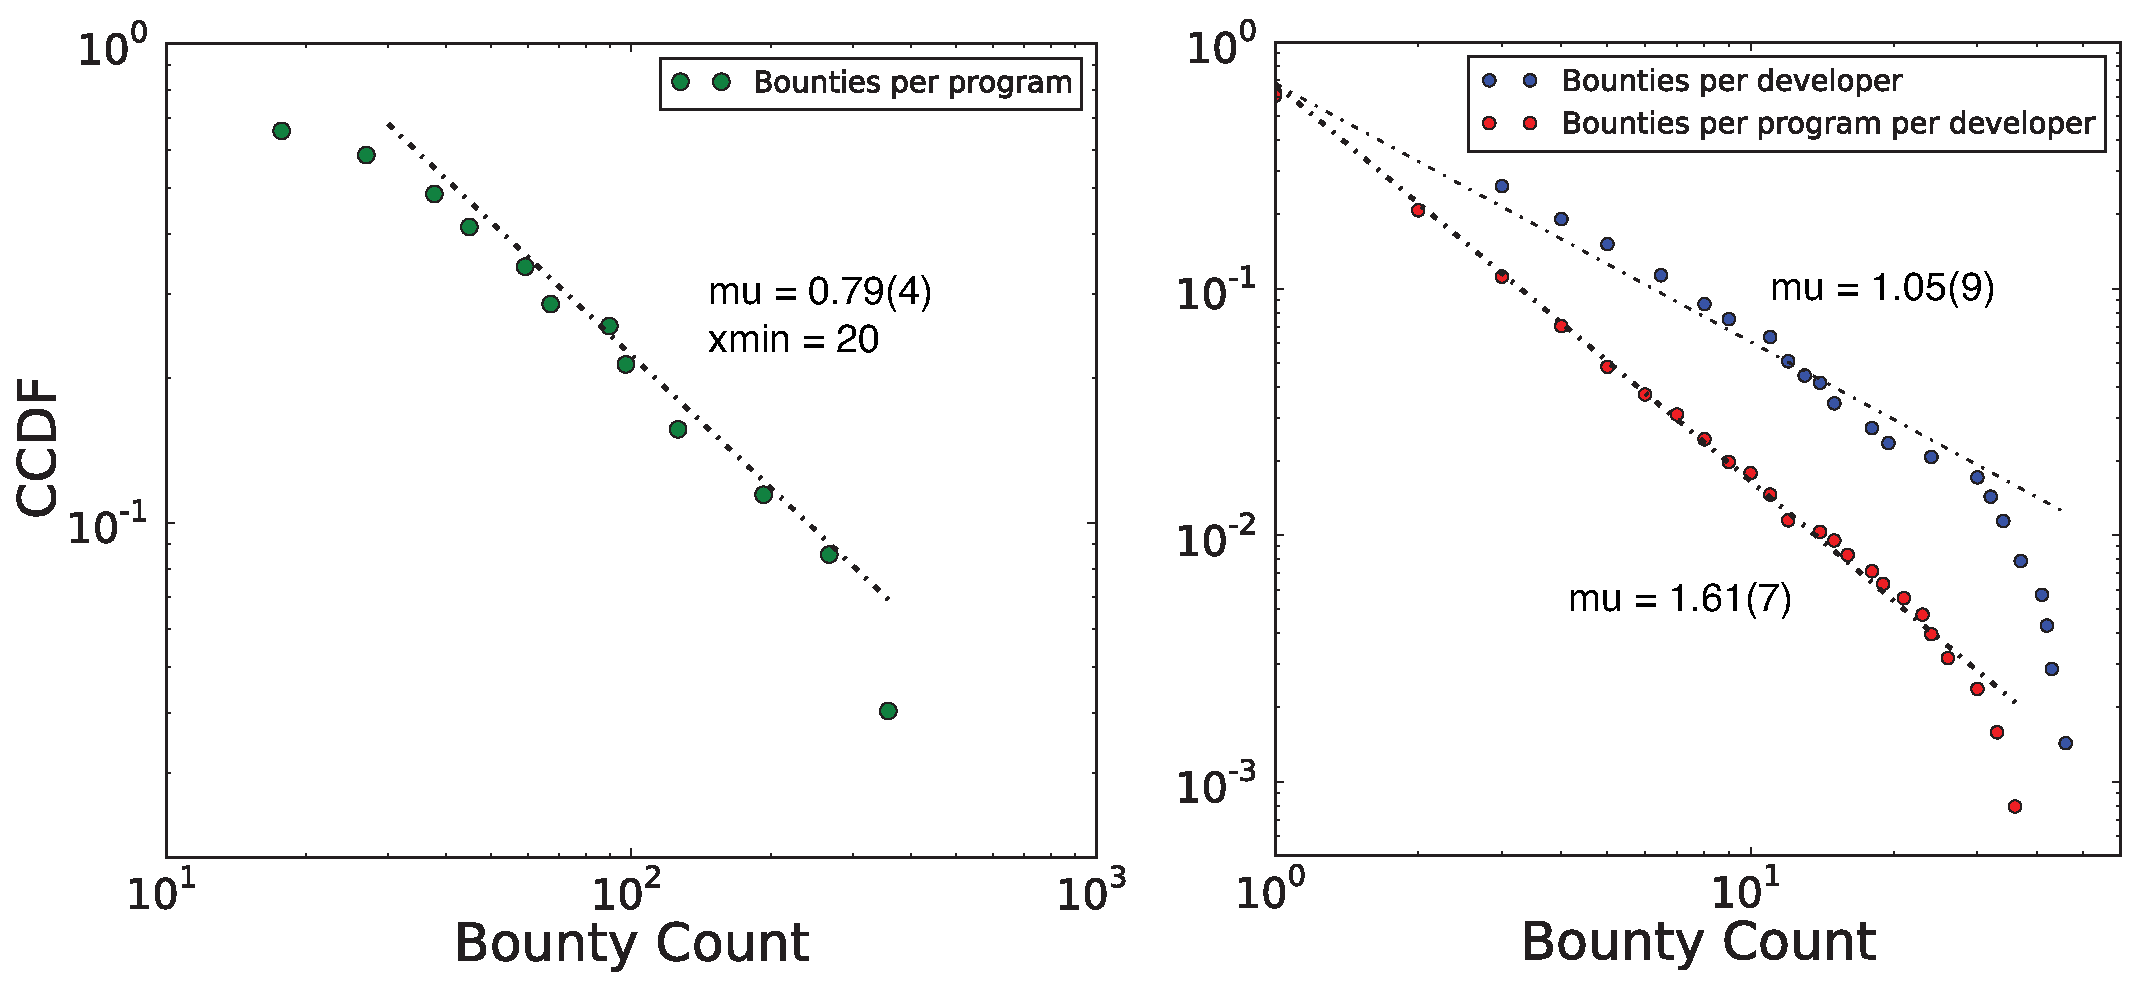
\includegraphics[width=12cm]{figures/CCDF_count_Bounties.eps}
\caption{}
\label{ }
\end{center}
\end{figure}


\begin{figure}
\begin{center}
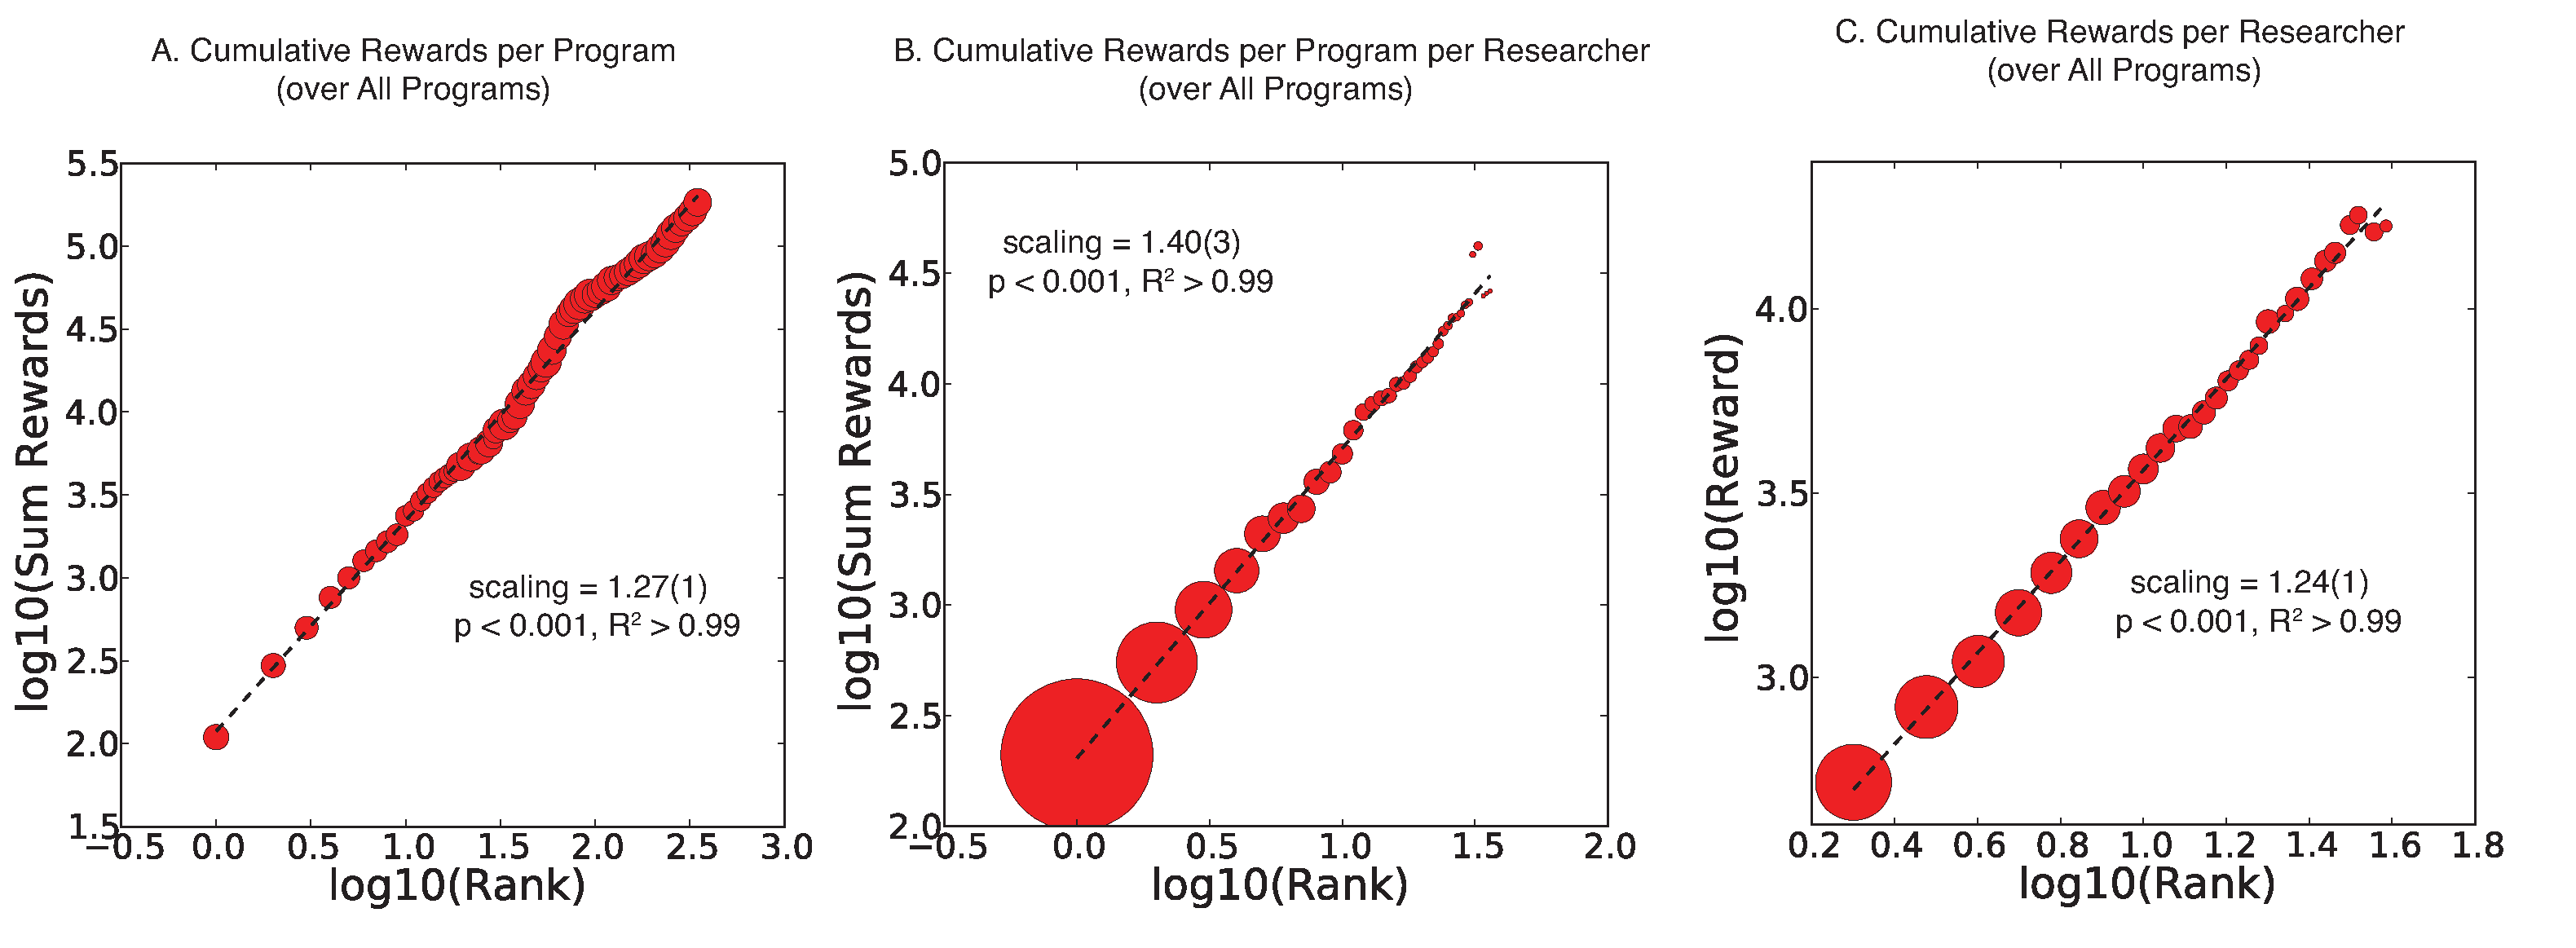
\includegraphics[width=16cm]{figures/scalings.eps}
\caption{}
\label{ }
\end{center}
\end{figure}
